\documentclass{beamer}
\usepackage[latin1]{inputenc}
\usepackage{hyperref}
\usetheme{Copenhagen}
%\usetheme{Singapore}
%\usetheme{Montpellier}
\title[RUM 2]{RUM 2 (RNA-Seq Unified Mapper)}
\bibliographystyle{unsrt}
\author{Mike DeLaurentis}
\institute{University of Pennsylvania}
\date{August 15, 2012}
\usepackage{listings}

\AtBeginSection[]
{
  \begin{frame}<beamer>
    \frametitle{Agenda}
    \tableofcontents[currentsection]
  \end{frame}
}

\begin{document}

\begin{frame}
\titlepage
\end{frame}

\begin{frame}{Agenda}
  \tableofcontents
\end{frame}

\section{Intro}

\begin{frame}{Who am I?}
  \begin{itemize}
  \item Working at Penn (ITMAT) since January
  \item Software engineering background
  \item Experience in a variety of languages, (Perl, Java, Clojure (lisp), Python, Ruby)
  \item ... and applications
  \end{itemize}
\end{frame}

\begin{frame}{What is RUM?}
  \begin{itemize}
  \item \textit{``RUM is an alignment, junction calling, and feature quantification pipeline specifically designed for Illumina RNA-Seq data''}
  \item Written by Gregory Grant (ggrant@grant.org)
  \item Runs on Linux / UNIX / Mac
  \item Can distribute work across multiple machines
  \end{itemize}
\end{frame}

\begin{frame}{What is RUM?}
  \begin{columns}
    \column{3in}
    \begin{description}
    \item [Inputs]
      \begin{itemize}
      \item RNA-Seq reads
      \item FASTA or FASTQ
      \item Paired or single
      \end{itemize}
    \item [Outputs]
      \begin{itemize}
      \item Unique and non-unique alignments
      \item Coverage plots
      \item Feature quantifications
      \item Junction calls
      \item List of novel inferred internal exons
      \end{itemize}
    \end{description}
    \column{2.5in}
    
\includegraphics[scale=0.4]{rumpouring2.png}
  \end{columns}
\end{frame}


\section{The RUM pipeline}

\begin{frame}{Phase 1: Preprocessing}

  \begin{itemize}
  \item Perform some quality checks on reads
  \item Split reads into N chunks
  \item Allows reads to be processed by N nodes on a cluster
  \end{itemize}

\end{frame}

\begin{frame}{Phase 2: Processing}

\begin{itemize}
  \item Align all reads against genome using Bowtie
  \item Align all reads against transcriptome using Bowtie
  \item Merge genome and transcriptome alignments and identify unmapped reads
  \item Align unmapped reads against genome using BLAT

  \item \textit{``This leverages the advantages of both genome and transcriptome mapping as well as combining the speed of Bowtie with the sensitivity and flexibility of Blat.''}

  \item Merge Bowtie and Blat alignments
\end{itemize}
\end{frame}

\begin{frame}{Phase 3: Postprocessing}

  \begin{itemize}
  \item Merge alignments for all chunks together
  \item Produce coverage plots, junction files
  \item Find novel internal exons
  \item Generate some reports
  \end{itemize}

\end{frame}

\section{Tour of the new RUM}

\begin{frame}{RUM 2 Goals}
  \begin{itemize}
  \item More code reuse for maintainability
  \item Improve inter-process communication
  \item More robust job state management
  \item Automated tests
  \end{itemize}
\end{frame}

\begin{frame}{Enhancements in RUM 2}
  \begin{itemize}
  \item Standard installation process
  \item New command-line interface
  \item Get status of running job
  \item Restart a job where it left off
  \item More reliable kill command
  \item Run a chunk or postprocessing by itself
  \item Relocatable indexes
  \item SAM file is closer to conforming to standard
  \end{itemize}
\end{frame}

\subsection{Installation}

\begin{frame}{Installing RUM}
  \begin{itemize}
  \item Uses standard Perl Makefile.PL
  \item Should be familiar to system administrators
  \item Download tarball from \texttt{https://github.com/PGFI/rum/downloads}
  \item \texttt{perl Makefile.PL}
  \item \texttt{make install} (optional)
  \item Then install indexes...
  \end{itemize}
\end{frame}

\begin{frame}{Installing Indexes}
  \begin{itemize}
  \item RUM needs an index for each organism you want to align against
  \item Index includes genome, gene annotations, and binary index files for Bowtie
  \item Run \texttt{rum\_indexes}; it will guide you through the process
  \end{itemize}
\end{frame}

\subsection{Command-line interface}

\begin{frame}{Command-line interface}

  Usage is \texttt{rum\_runner ACTION [OPTIONS]} where action is one of:

  \begin{itemize}
  \item \texttt{align} - Run an alignment
  \item \texttt{status} - Check the status of a job
  \item \texttt{stop} - Stop a job (can be restarted later)
  \item \texttt{kill} - Stop a job and clean it up (to restart from scratch)
  \item \texttt{clean} - Remove output files for a job
  \item \texttt{help} - Get help
  \item \texttt{version} - Show version number
  \end{itemize}

\end{frame}

\begin{frame}[fragile]{Running an alignment}
Use \texttt{rum\_runner align} to run an alignment:
\begin{verbatim}
rum_runner align \
  --output dir \
  --index  ~/rum_indexes/hg19 \
  --name   TestJob \
  --chunks 25 \
  ~/samples/forward.fq ~/samples/reverse.fq
\end{verbatim}
\end{frame}

\subsection{Job state management}

\begin{frame}[fragile]{Job status}
  \begin{itemize}
  \item Use \texttt{rum\_runner status} to check on the status of a
    running job.
  \end{itemize}
  \tiny
\begin{verbatim}
Processing in 25 chunks
-----------------------
XXXXXXXXXXXXXXXXXXXXXXXXX Run bowtie on genome
XXXXXXXXXXXXXXXXXXXXXXXXX Parse genome Bowtie output
X XXX  XX XX XXXX  XXXXX  Run bowtie on transcriptome
X XXX  XX XX XXXX  XXXXX  Parse transcriptome Bowtie output
X XXX  XX XX XXXX  XXXXX  Merge unique mappers together
X XXX  XX XX XXXX  XXXXX  Merge non-unique mappers together
X XXX  XX XX XXXX  XXXXX  Make unmapped reads file for blat
X XXX  XX XX XXXX  XXXXX  Run blat on unmapped reads
X XXX  XX XX XXXX  XXXXX  Run mdust on unmapped reads
X XXX  XX XX XXXX  XXXXX  Parse blat output
X XXX  XX XX XXXX  XXXXX  Merge bowtie and blat results
X XX   XX XX  XXX   XXXX  Clean up RUM files
X XX   XX XX  XXX   XXXX  Produce RUM_Unique
X XX   XX XX  XXX   XXXX  Sort RUM_Unique by location
X X    XX XX  XXX   XXXX  Sort cleaned non-unique mappers by ID
X X    XX XX  XXX   XXXX  Remove duplicates from NU
X X    XX XX  XXX   XXXX  Create SAM file
X X    XX XX  XXX   XXXX  Create non-unique stats
X X    XX XX  XXX   XXXX  Sort RUM_NU
X X    XX XX  XXX   XXXX  Generate quants
...
\end{verbatim}
\end{frame}

\begin{frame}[fragile]{Job status}
\tiny
\begin{verbatim}
Postprocessing
--------------
X Merge RUM_NU files
X Make non-unique coverage
X Merge RUM_Unique files
X Compute mapping statistics
X Make unique coverage
X Finish mapping stats
X Merge SAM headers
X Concatenate SAM files
X Merge quants
  make_junctions
  Sort junctions (all, bed) by location
  Sort junctions (all, rum) by location
  Sort junctions (high-quality, bed) by location
  Get inferred internal exons
  Quantify novel exons

All the chunk error log files are empty. That's good.
Main error log file is empty. That's good.

RUM is running (job ids 815718, 815720).
\end{verbatim}
\end{frame}

\begin{frame}{Job state management}
  \begin{itemize}
  \item Model the workflow as a state machine
  \item A completed step transitions the job from one state to another
  \item Stitch steps together into a workflow
  \item Determine the state of a job by looking at which output
    files exist
  \item Similar to GNU Make (but simpler)
  \item Basis for a lot of additional features
  \end{itemize}
\end{frame}

\begin{frame}{Recovering from errors}
  \begin{columns}[c]
    \column{2in}
    
\includegraphics[scale=0.2]{success.jpg}
    \column{2.5in}
    \begin{itemize}

    \item In case of failure...

    \item RUM 2 allows easier recovery

    \item Running ``\texttt{rum\_runner align}'' again, RUM will determine what state the job was in when it failed

    \item Just resumes at the next uncompleted step

    \item Can save \textit{a lot} of time when recovering from infrastructure failure

    \end{itemize}

  \end{columns}
\end{frame}

\begin{frame}[fragile]{Killing a job}
\begin{itemize}
\item To stop a job and remove all of its output:
\begin{verbatim}
  rum_runner kill -o dir
\end{verbatim}
\item Useful if you've run a job with incorrect parameters and need to start over
\end{itemize}
\end{frame}

\subsection{Work distribution}

\begin{frame}{Work distribution}
  \begin{columns}
    \column{2.5in}
    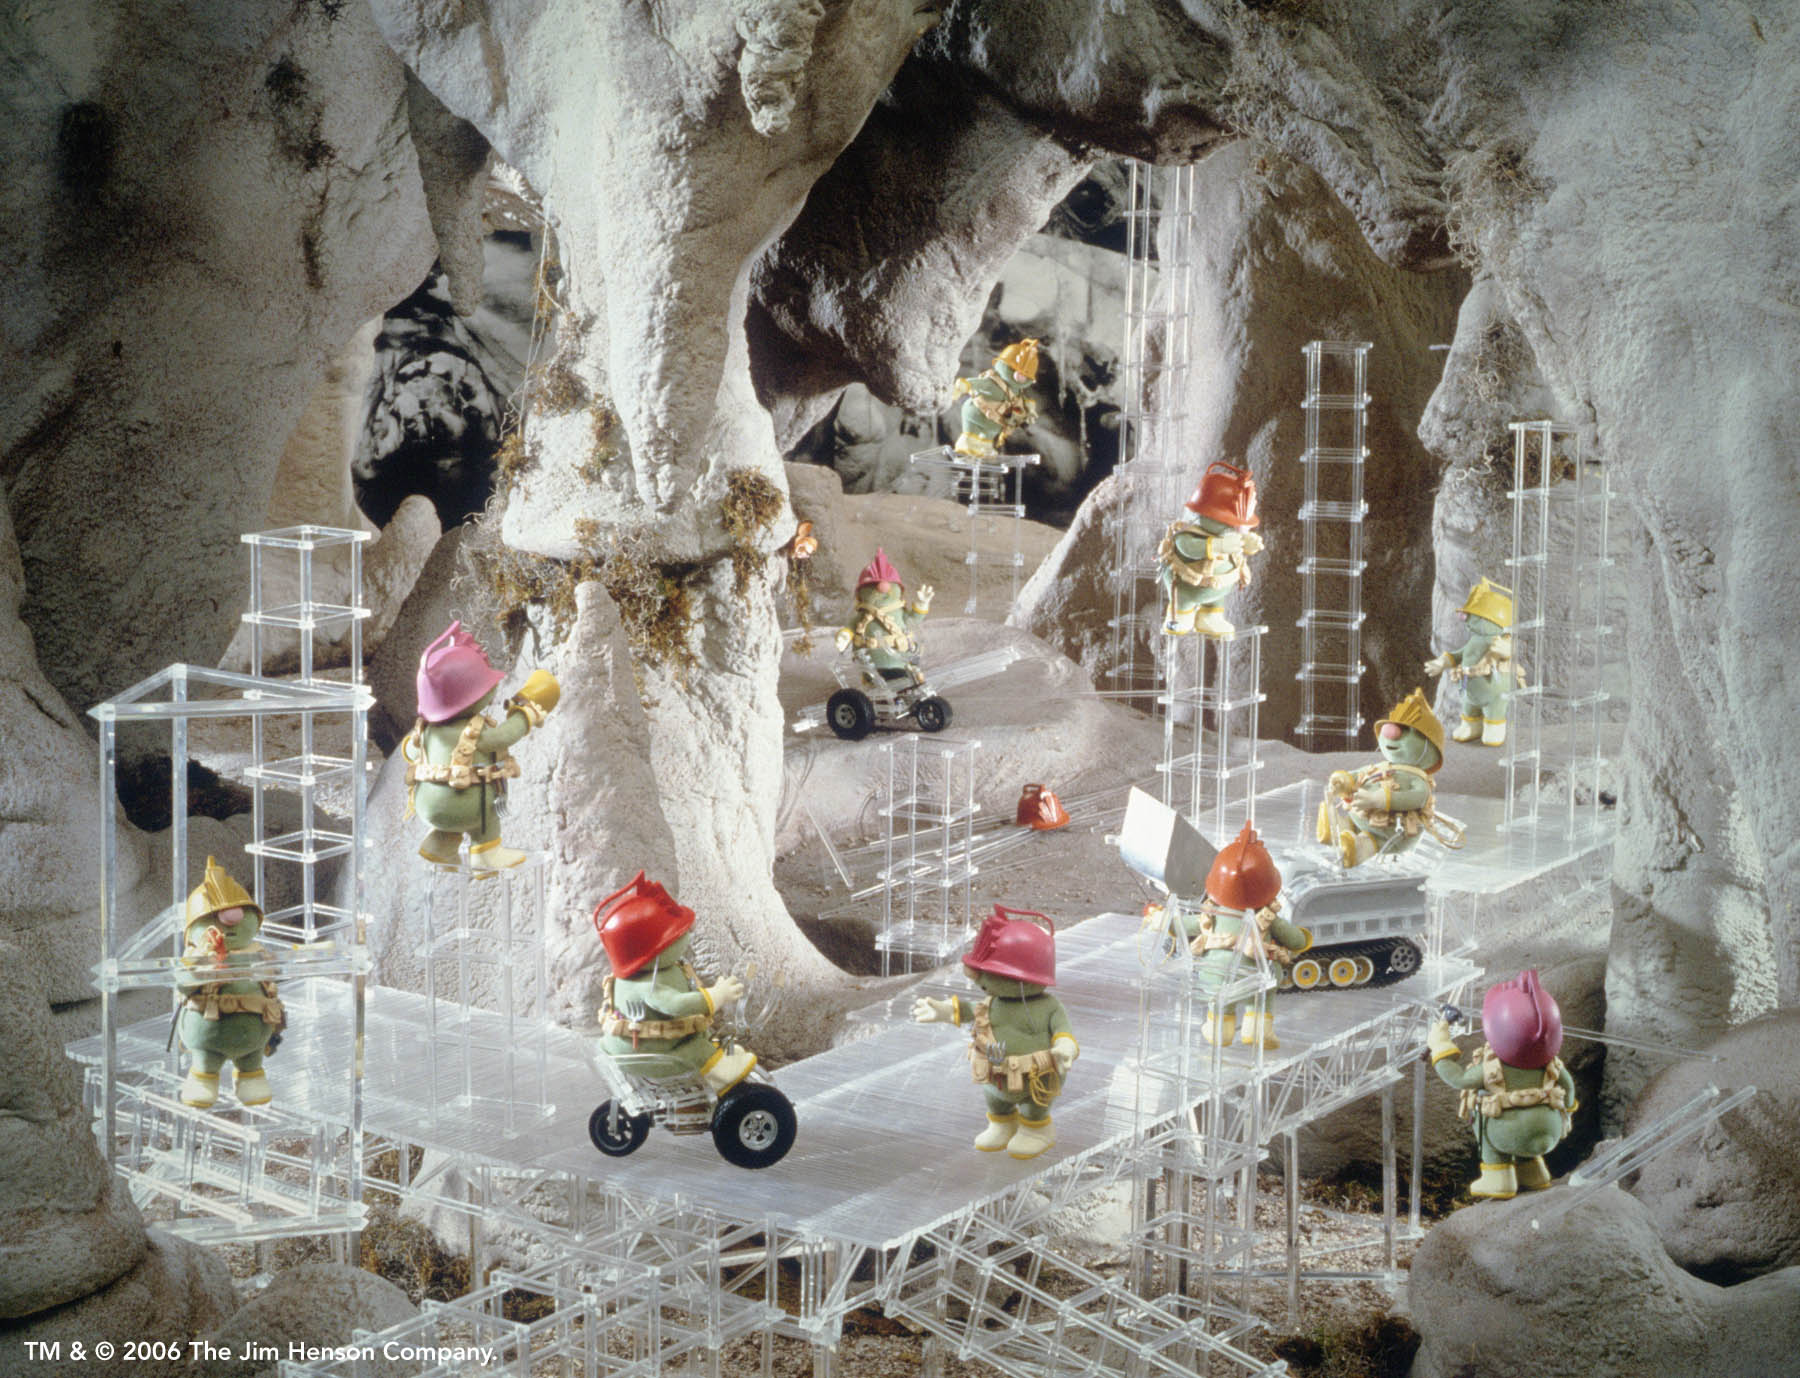
\includegraphics[scale=0.4]{doozers.jpg}    
    \column{2.5in}
    \begin{itemize}
    \item Automatic support for one multi-core machine (will run each chunk in a separate process by default)
    \item Built-in support for Sun Grid Engine, with \texttt{--qsub} option
    \item Easily extensible for other platforms
    \end{itemize}
  \end{columns}
\end{frame}

\begin{frame}[fragile]{Work distribution}

For other platforms, you can either extend a Perl class to provide
support, or set up some scripts to run the parts of the job on
different machines:

\pause

\begin{itemize}
\item  Run preprocessing alone:

\begin{verbatim}
rum_runner -o <dir> --preprocess
\end{verbatim}

\pause

\item Run chunks one at a time:

\begin{verbatim}
rum_runner -o <dir> --process --chunk 8
\end{verbatim}

\pause

\item Run postprocessing alone:

\begin{verbatim}
rum_runner -o <dir> --preprocess
\end{verbatim}

\end{itemize}

\end{frame}

% http://tomboythatwearsmakeup.com/wp-content/uploads/2011/03/dz_fr_012-1.jpg

\section{Web resources}

\begin{frame}{Web resources}
  \begin{description}
    \item [Main github page] 
      \url{https://github.com/PGFI/rum}

    \item [User guide] 
      \url{https://github.com/PGFI/rum/wiki}

    \item [Issues] 
      \url{https://github.com/PGFI/rum/issues}

    \item [Downloads] 
      \url{https://github.com/PGFI/rum/downloads}
    
  \end{description}
\end{frame}

\section{Demo}

%\subsection{User guide}

%\centering
%\begin{frame}{User guide}
%  \url{https://github.com/PGFI/rum/wiki}
%  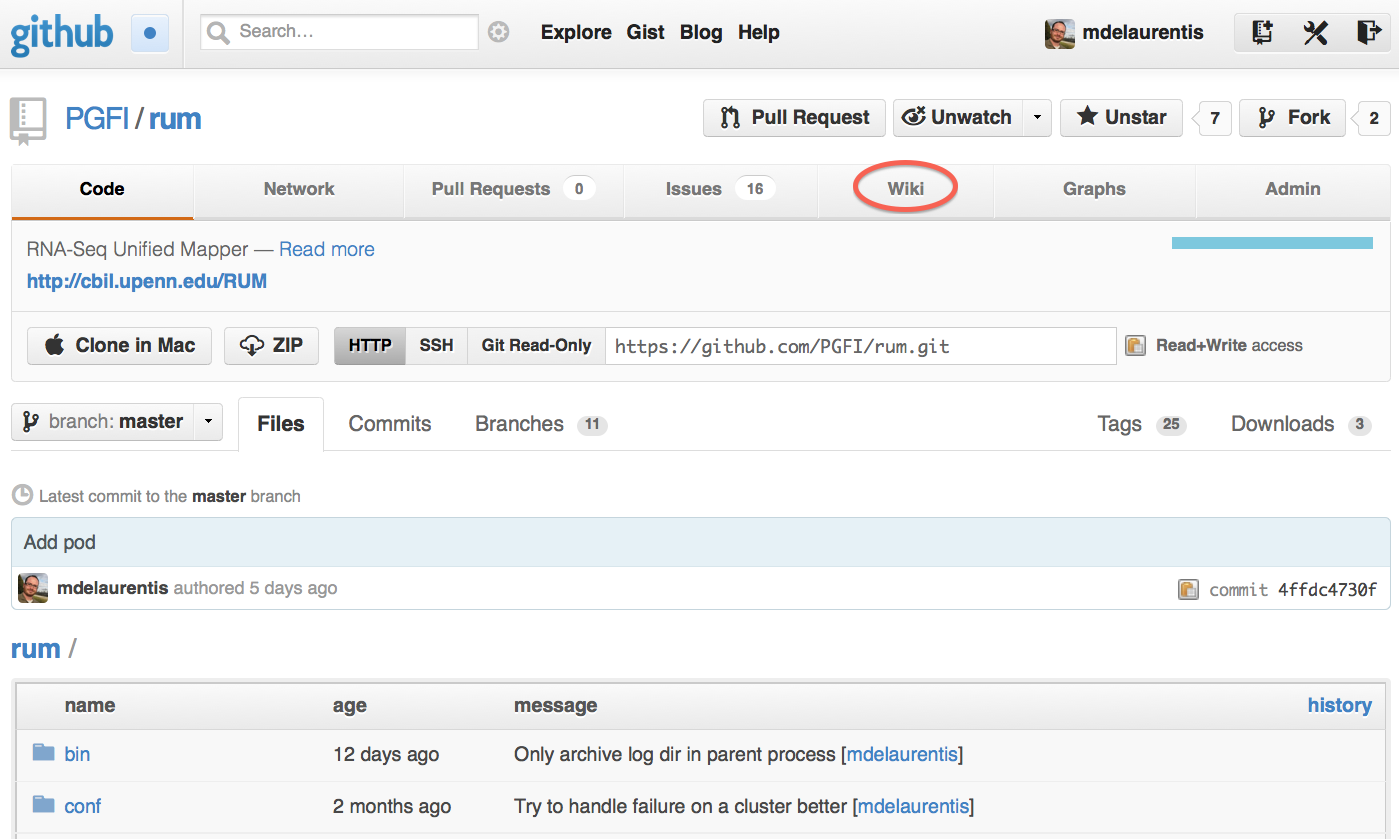
\includegraphics[scale=0.2]{github-main-wiki.png}
%\end{frame}

%\centering
%\begin{frame}{User guide}
%  \url{https://github.com/PGFI/rum/wiki}
%  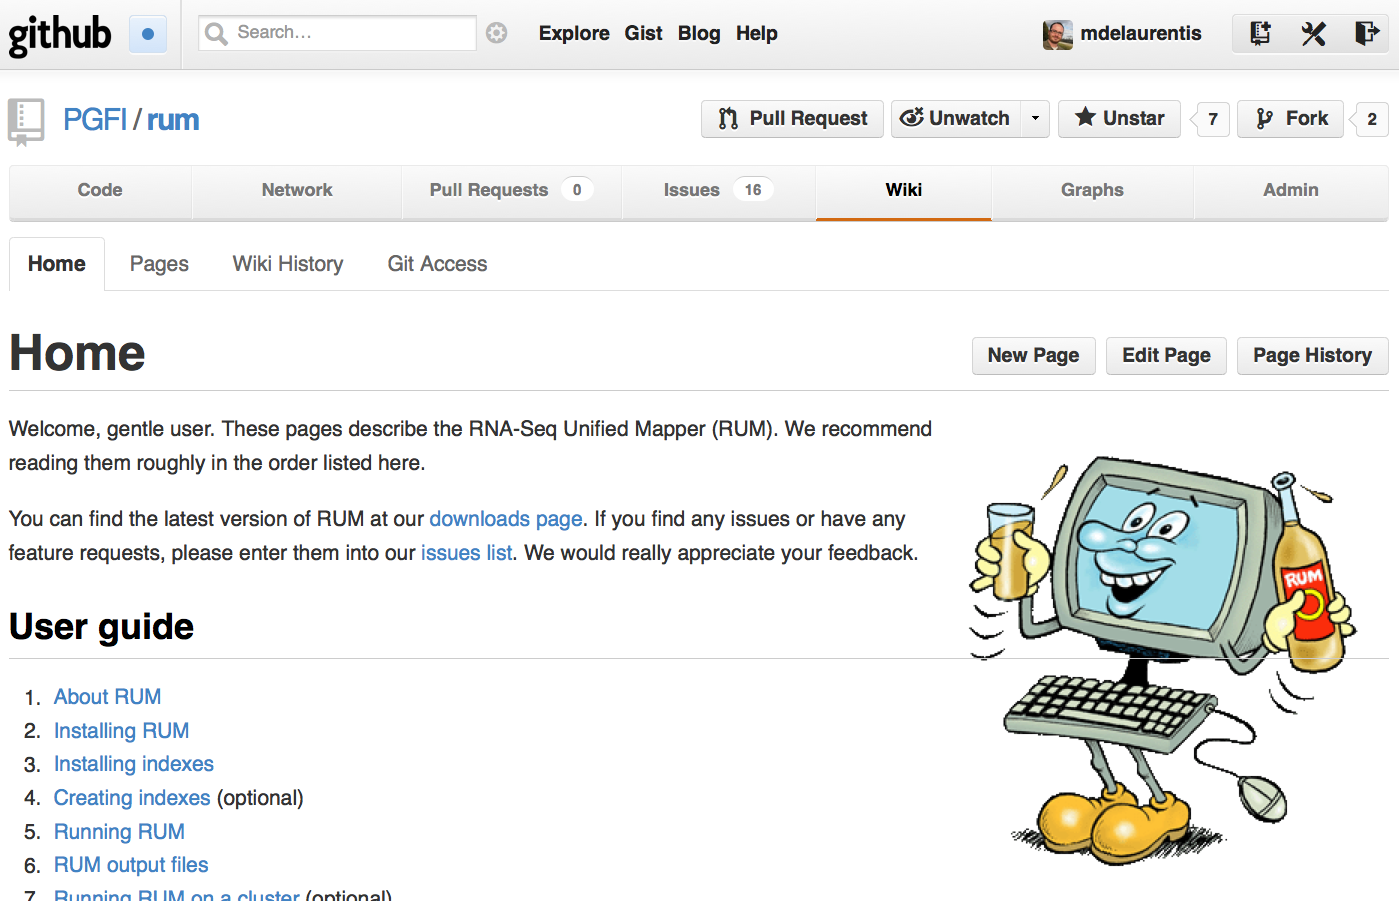
\includegraphics[scale=0.2]{github-wiki.png}
%\end{frame}

%\subsection{Downloads}

%\centering
%\begin{frame}{Downloads}
%  \url{https://github.com/PGFI/rum/downloads}
%  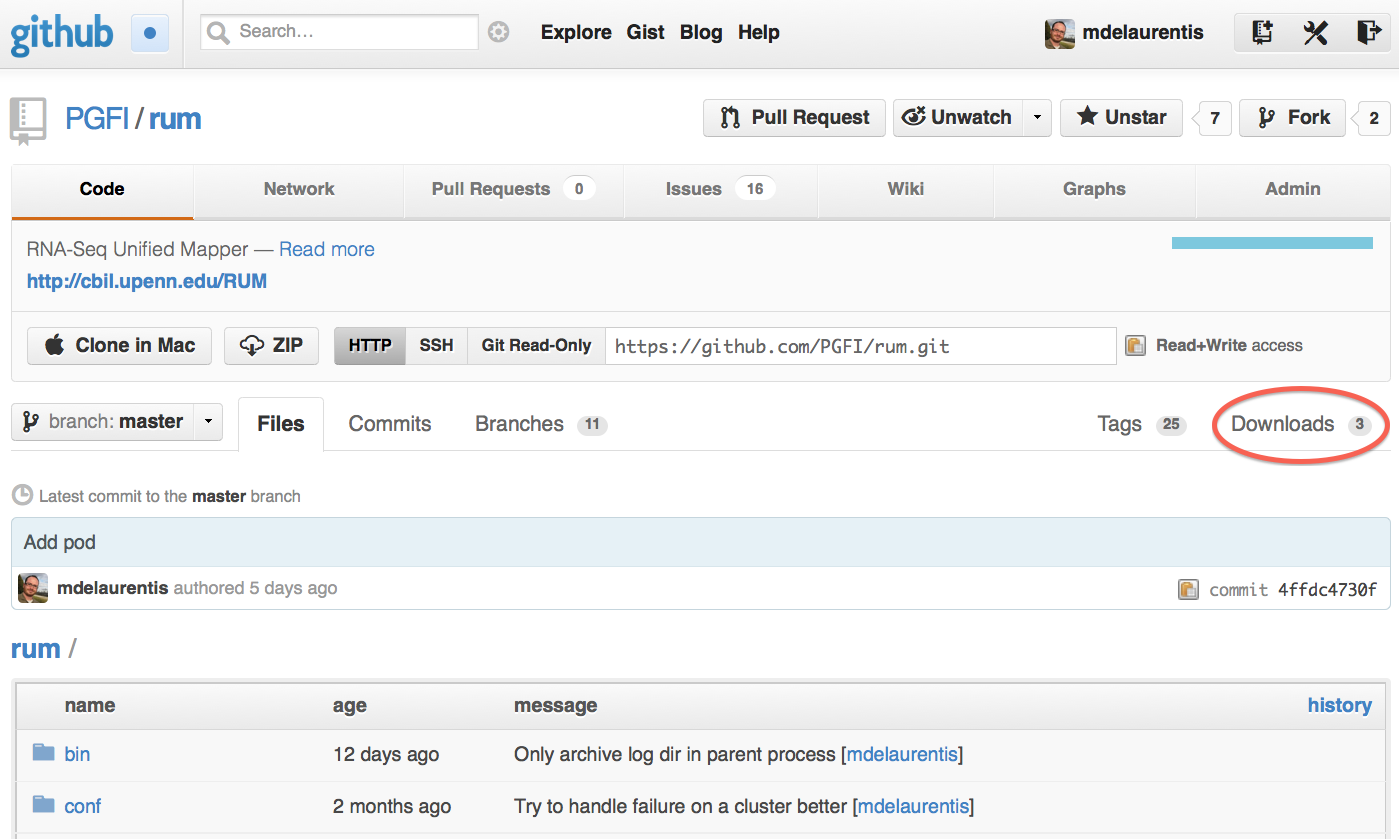
\includegraphics[scale=0.2]{github-main-downloads.png}
%\end{frame}

%\centering
%\begin{frame}{Downloads}
%  \url{https://github.com/PGFI/rum/downloads}
%  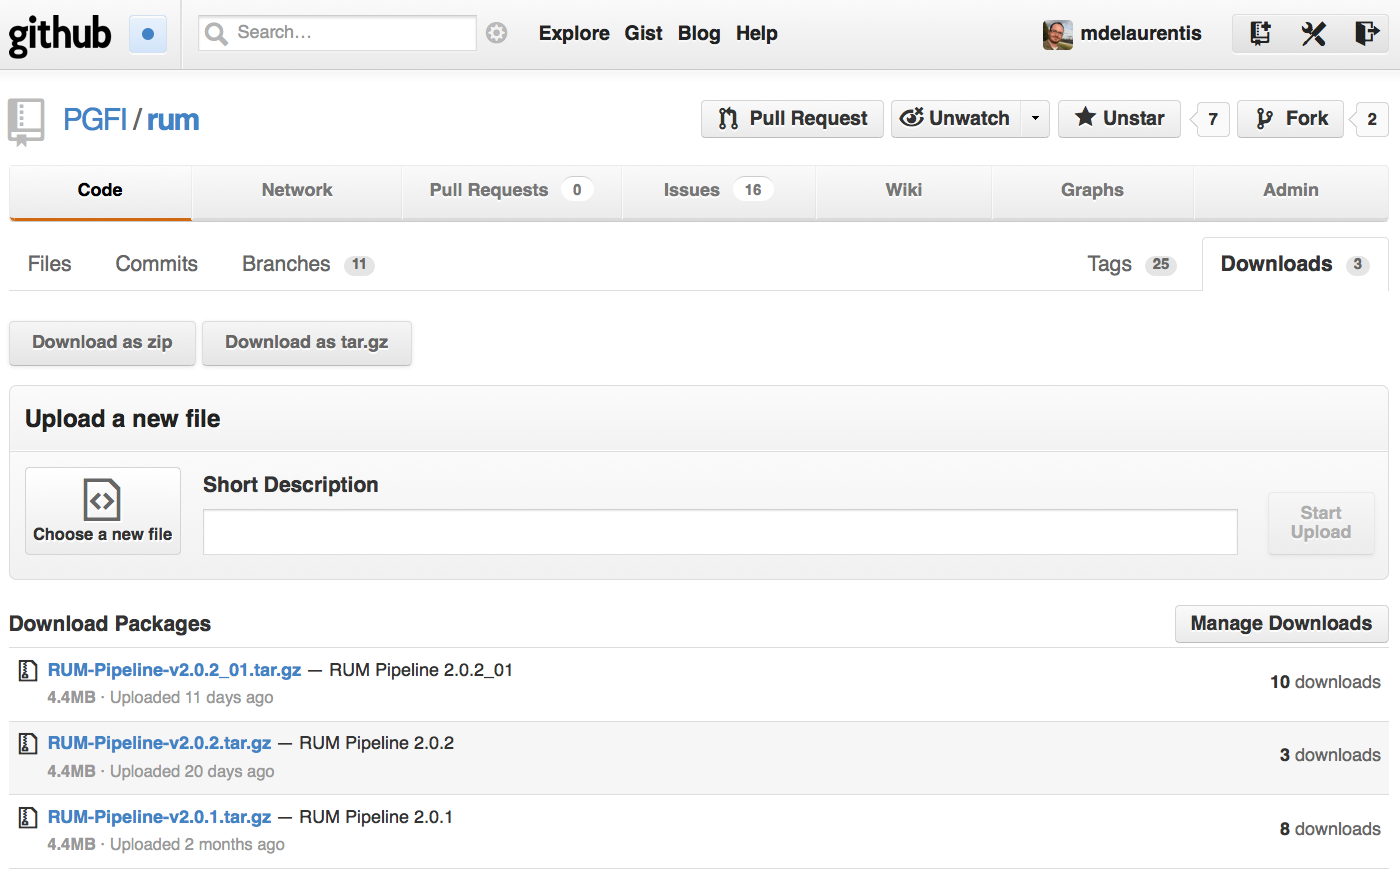
\includegraphics[scale=0.2]{github-downloads.png}
%\end{frame}

%\subsection{Issues}

%\centering
%\begin{frame}{Issues}
%  \url{https://github.com/PGFI/rum/issues}
%  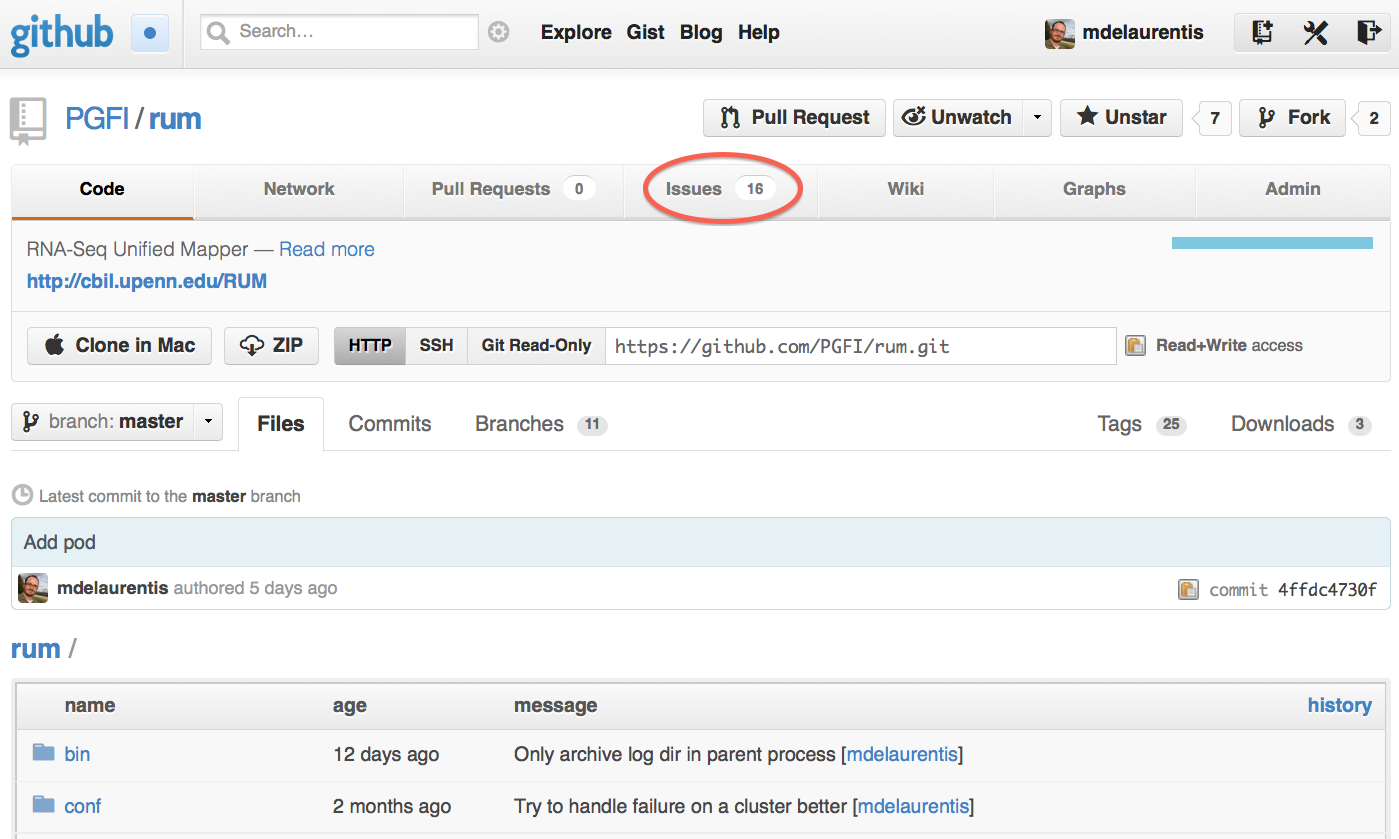
\includegraphics[scale=0.2]{github-main-issues.png}
%\end{frame}

%\centering
%\begin{frame}{Issues}
%  \url{https://github.com/PGFI/rum/issues}
%  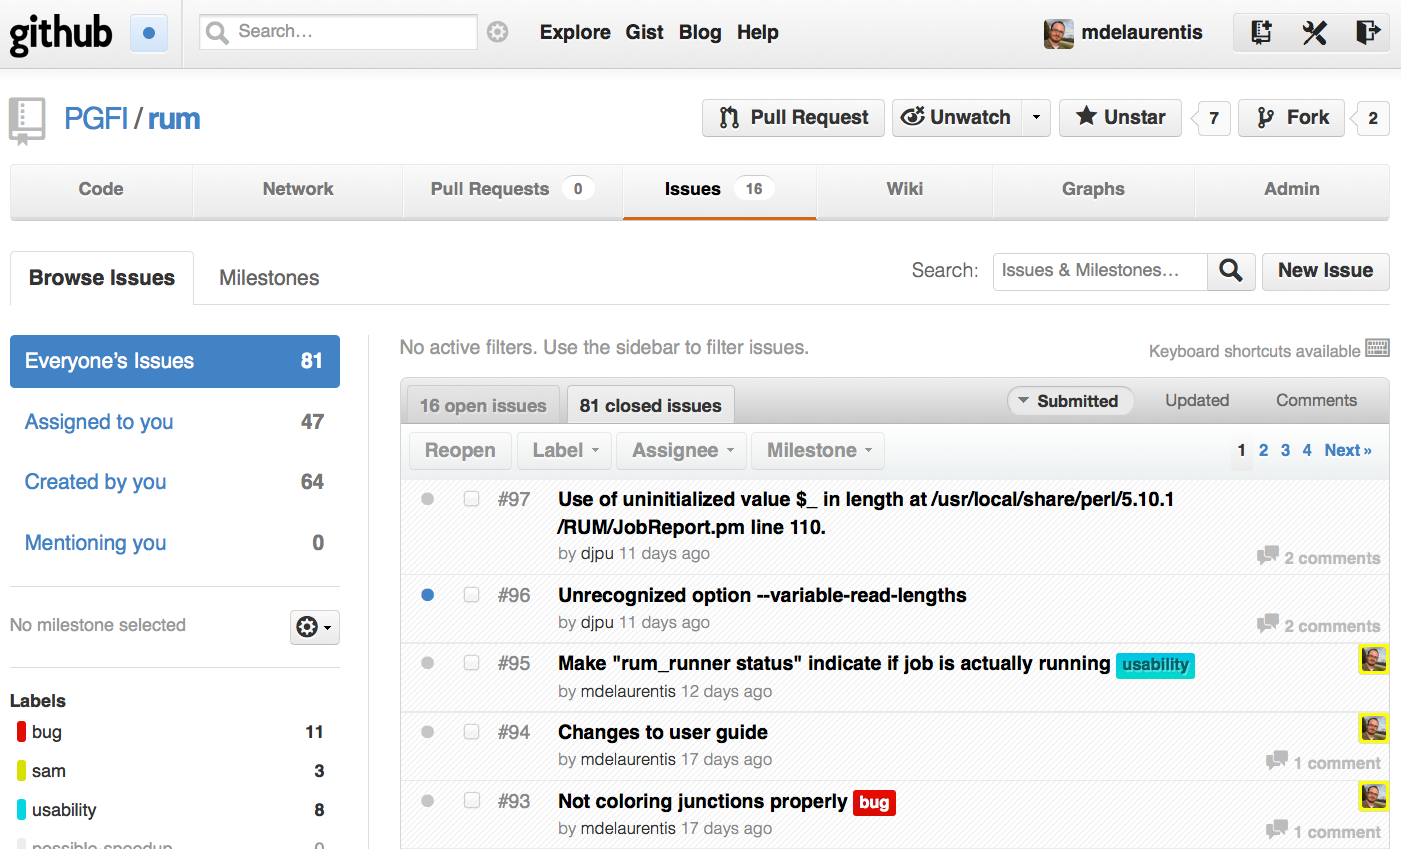
\includegraphics[scale=0.2]{github-issues.png}
%\end{frame}

%\section{Future direction}

%\begin{frame}{Possible future enhancements}
%  \begin{itemize}
%  \item Use original read names throughout the pipeline
%  \item Performance improvements
%  \end{itemize}
%\end{frame}



\end{document}
